\bf{Пример}

Пусть $ H=2, W=3, R=[0,1,1,0,0,1], C=[0,0,1,1,2,2], $ и $ Q=2. $ 

Проверяющий модуль \bf{(grader)} вызывает \t{give_initial_chart(2, 3, [0, 1, 1, 0, 0, 1], [0, 0, 1, 1, 2, 2]). }

Исходно распределение участников по посадочным местам выглядит следующим образом.

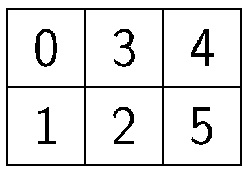
\includegraphics{image-000.jpg}

Пусть затем проверяющий модуль вызывает \t{swap_seats(0, 5).} После запроса $ 0 $ распределение участников по посадочным местам выглядит следующим образом.

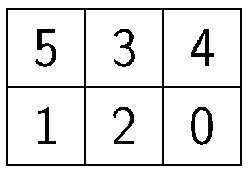
\includegraphics{image-001.jpg}

Множества посадочных мест, соответствующие множествам участников $ \{0\}, \{0,1,2\}, $ и $ \{0,1,2,3,4,5\} $ являются красивыми прямоугольниками. Следовательно, красота этого распределения участников по посадочным местам равна $ 3 $ , и функция \t{swap_seats }должна вернуть $ 3 $ . 

Пусть теперь проверяющий модуль снова вызывает \t{swap_seats(0, 5)}. После запроса $ 1 $ распределение участников по посадочным местам возвращается к исходному состоянию. Множества посадочных мест, соответствующие множествам участников $ \{0\}, \{0,1\}, \{0,1,2,3\} $ и $ \{0,1,2,3,4,5\} $ являются красивыми прямоугольниками. Таким образом, красота этого распределения участников по посадочным местам равна $ 4 $ , и функция \t{swap_seats }должна вернуть $ 4 $ . 

Файлы \t{sample-01-in.txt} и \t{sample-01-out.txt} в приложенном zip-архиве соответствуют этому примеру. В архиве есть также другие примеры ввода и вывода.
